\section{Introduction}

As the scientific community began to address problems involving sequentially structured data, RNNs returned to the forefront, leading to the development of new designs such as GRUs. However, it became apparent that RNNs had difficulty handling very long sequences. To address this problem, the Attention model was introduced as an auxiliary module, significantly improving performance in complex tasks such as image captioning and neural machine translation.

The concept of the Attention model initially found application in models that combined CNN and RNN, and then was incorporated into Transformers, the model underlying tools such as ChatGPT. This led to the emergence of an inevitable question, "\textit{Do we really need RNN and Attention models together for sequencing tasks, or can one Attention model suffice on its own?}" This question prompted the exploration of sequence models without the use of RNNs.

In this section, we will explore how this change came about through innovations implemented in the \textbf{Image Captioning} and \textbf{Machine Translation} tasks.


\section{Caption Model}

\subsection{Show and Tell}
Image captioning is the process of generating a textual description for given images. It can be seen as a Sequence to Sequence problem from beginning to end, where images, considered as sequences of pixels, are transformed into sequences of words. This task requires processing both textual and image statements. For the textual part, we use recurrent neural networks (RNNs) and for the visual part, we use convolutional neural networks (CNNs) to obtain feature vectors. Specifically, the architecture developed by Google in 2014 in the paper \href{https://arxiv.org/pdf/1411.4555}{"Show and Tell: A Neural Image Caption Generator" (Bengio et al.)} uses both GoogleNet and LSTM.

The procedure begins with feature extraction of the image using GoogleNet, which produces a feature vector, denoted as $I$. This vector is then inserted into the LSTM sequence at time $t=-1$, only once. Next, starting at $t=0$, a sequence of word vectors is inserted. Each word is represented as a one-hot vector $S_t$ with dimensions equal to the size of the vocabulary.

At each time step, the word vector $S_t$ is transformed through an embedding layer $W_e S_t$ and provided to the LSTM. Then, the input is processed along with the previous hidden state to produce a new hidden state and calculate the probability $p_t$ of the next word in the sequence. The word with the highest probability, denoted as $\log p_t(S_{t+1})$, is chosen as the output for that time step. This process is repeated until a special end-of-sentence word ($S_N$) or a maximum length of the sequence is reached. Check the image below for a visual representation of the process:
\newpage

\begin{figure}[!htbp]
    \centering
    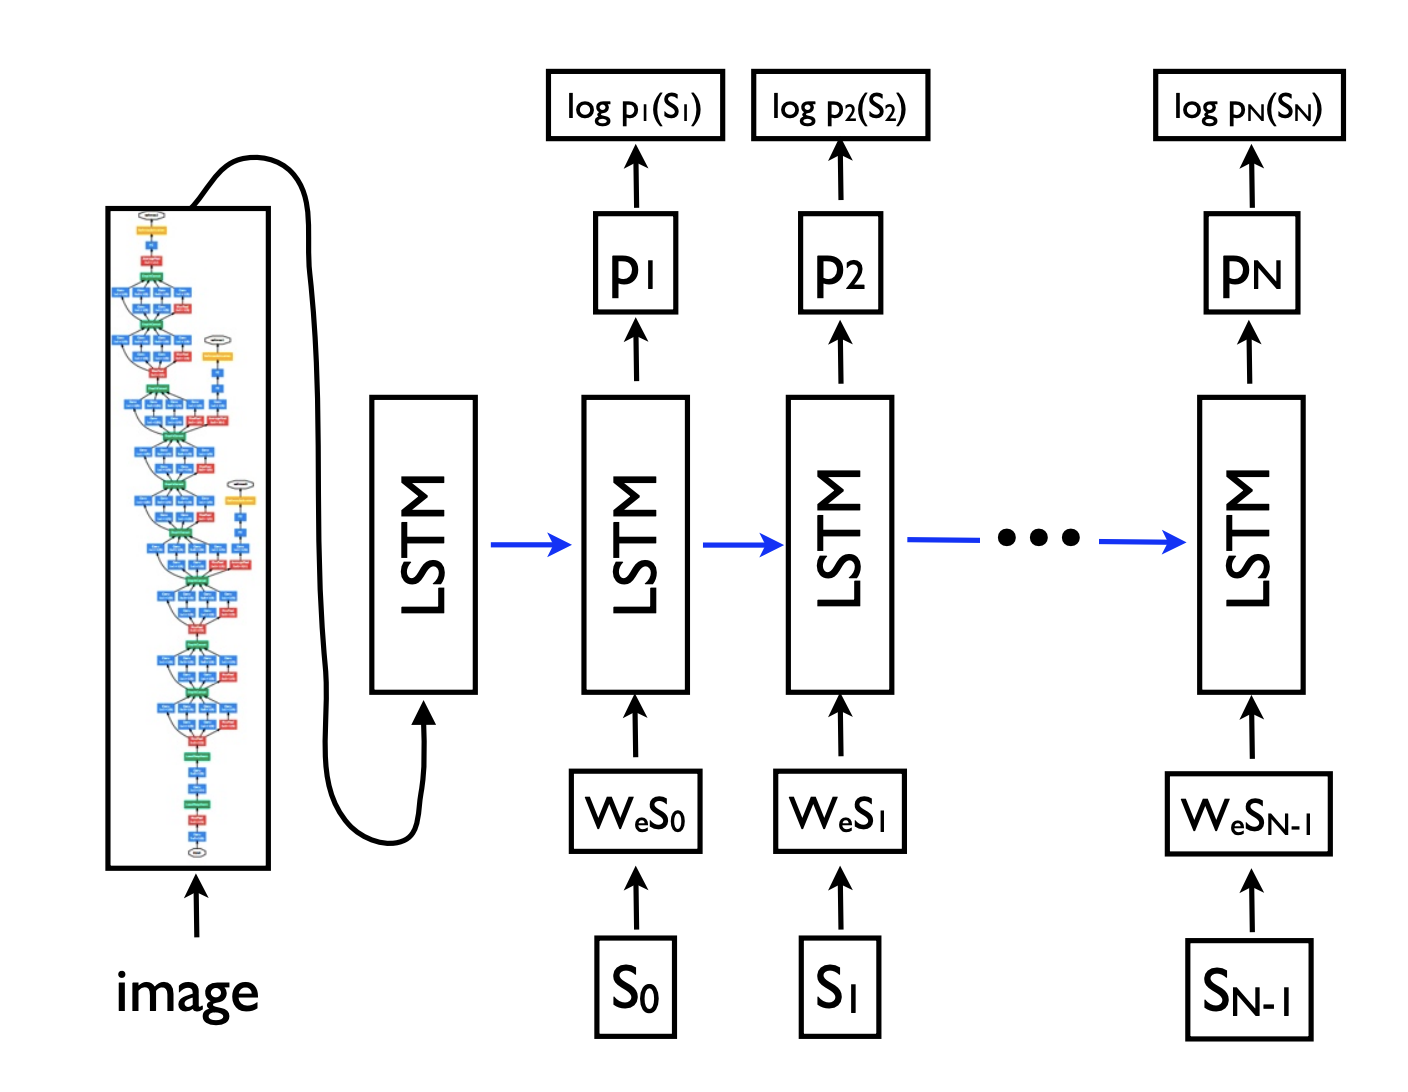
\includegraphics[width=\linewidth]{tikz/chapter7 - Show and Tell Model.png}
    \caption{{\color{red}\colorbox{pink}{Tikz TO-DO}} Show and Tell Caption Model}
\end{figure}

The quality of the generated caption depends strongly on the performance of the CNN, making fine-tuning crucial. So, the architecture combines CNN and LSTM in a way that leverages the visual feature extraction capabilities of CNN and the sequential modeling capabilities of LSTM to generate accurate and consistent captions for images.

For inference time, the model uses one of the following methods: \textbf{Sampling} and \textbf{Beam Search}.

In the sampling method, the first word is extracted according to a probability $p_1$, then the corresponding embedding is provided as input and the next word is extracted with probability $p_2$ (which depends on the probability that a certain word has been predicted previously). This process continues until the special end-of-sentence token is extracted or a maximum length is reached.

\begin{figure}[!htbp]
    \centering
    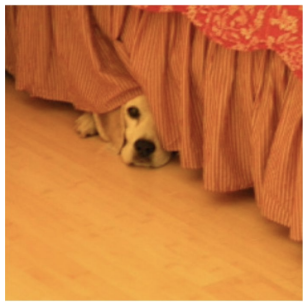
\includegraphics[width=\linewidth]{tikz/chapter7 - Sampling.png}
    \caption{{\color{red}\colorbox{pink}{Tikz TO-DO}} Sampling Visual Example}
\end{figure}

With Beam Search, on the other hand, we iteratively consider the \textbf{$k$ best sentences up to time $t$} as candidates to generate sentences of length $t+1$, keeping only the $k$ best of them. This approach allows more word combinations to be explored, improving the quality of the generated sentences compared to simple sampling.

\begin{figure}[!htbp]
    \centering
    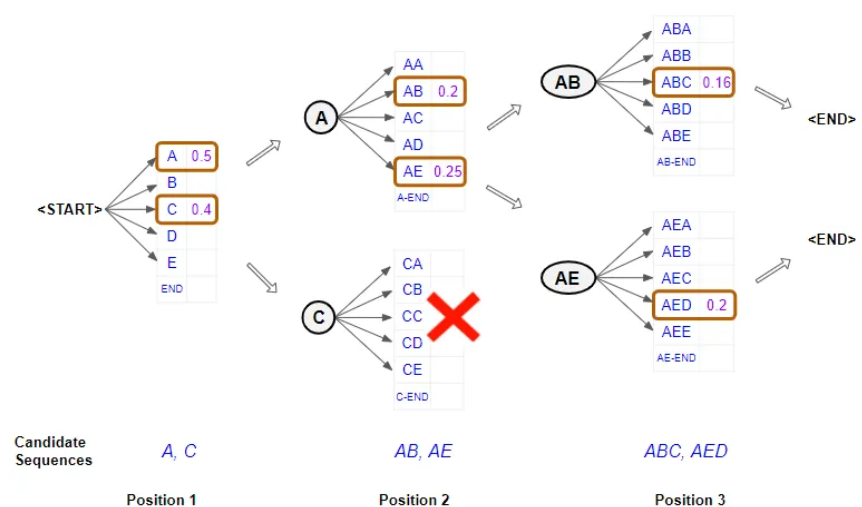
\includegraphics[width=\linewidth]{tikz/Beam Search.png}
    \caption{{\color{red}\colorbox{pink}{Tikz TO-DO}} Beam Search Visual Example}
\end{figure}

In the image above you can see an example of Beam Search with a width of 2, using characters for simplicity. Here's the description of what is happening:
\begin{itemize}
    \item \textbf{First Position}: The model starts with the token "<START>" and calculates the probabilities for each possible word. It selects the two characters with the highest probability, for example "A" and "C". 
    \item \textbf{Second position}: The model generates the probabilities for the second position twice, holding the first position ("A" or "C") constant. It then chooses the two best pairs of characters based on the combined probability, such as "AB" and "AE."
    \item \textbf{Third position}: This process is repeated. The model calculates the probabilities for the third position, limiting the first two positions to "AB" or "AE," and selects the best three combinations of characters based on the combined probability of the first three characters. This continues until a token "<END>" is selected, marking the end of that branch of the sequence. Simple, isn't it? \faSmile[regular]
\end{itemize}

In order to test the performance of the model, we face the challenge of comparing the output of the model with the \textbf{captions of human annotators}. Of course, the annotations of different individuals may vary, presenting inherent discrepancies. To address this problem, the Bilingual Evaluation Understudy (BLEU) score was used.

\subsection{BLEU Score}

The BLEU score is a metric used to evaluate the quality of texts generated in natural language processing (NLP) models. The text generated by the model is called \textbf{Candidate}, while the possible correct texts are called \textbf{References}. The BLEU score compares the candidate with the references to measure their similarity.

The BLEU score ranges from 0 to 1 and is based on accuracy, i.e., the \textbf{proportion of matching n-grams with references} (sequences of n words) found in the candidate compared \textbf{to the total number of n-grams in the candidate}. Usually, n-grams of size 1 to 4 are considered.

To prevent the candidate from scoring well by repeating the same n-gram many times, we \textbf{limit the number of occurrences} of each n-gram in the references. For example, if a reference contains the word "the" twice, the candidate should also not have more than two occurrences of "the".

Finally, the BLEU score is multiplied by a \textbf{brevity penalty} to prevent translations that are too short from getting high scores. 

Example:

\; The Reference is: "\textit{Transformers: Transformers make everything quick and efficient.}" 

\; The Candidate is: "\textit{Transformers Transformers Transformers Transformers.}" \ \img{tikz/chapter7 - Optimus Prime.png}
 
The BLEU score is low because the candidate repeats "Transformers" without providing full context, while the reference has a meaningful sentence. 

\section{Captioning with Attention}

\subsection{Show, Attend and Tell}

Captioning with attention represents a significant innovation in the field, especially for image and text processing. This approach, which was introduced in the paper \href{https://arxiv.org/pdf/1502.03044}{"Show, Attend and Tell: Neural Image Caption Generation with Visual Attention" (Xu et al.)} in 2015, has overcome some limitations of previous models, paving the way for more advanced results in image processing and caption generation.

The key idea of this approach is the integration of two key components: a convolutional neural network (CNN) for image feature extraction and a recurrent neural network (RNN) with an attention mechanism to generate captions. This combination allows the model to \textbf{focus attention on specific parts of the image while generating the corresponding description}.

The main innovations introduced by this approach are as follows:

\begin{itemize}
    \item \textbf{Feature Extractor}: A CNN is used to extract a set of feature vectors, each of which represents a part of the image. So, here we maintain the spatial information.
    \item \textbf{RNN with Attention}: The extracted feature maps are not only used for initializing the RNN, but are passed to each cell of the RNN during caption generation. This approach allows the network to focus attention on specific parts of the image as it generates each caption word. Each RNN cell produces both the probability of the predicted word ($p(y_t)$) and an attention map ($\alpha_t$) indicating the relevant parts of the image.
\end{itemize}

\begin{figure}[!htbp]
    \centering
    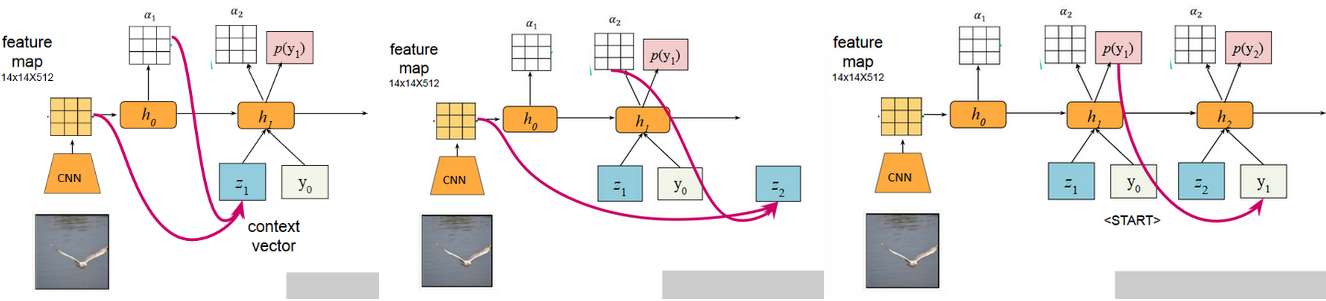
\includegraphics[width=1\linewidth]{tikz/Attention Model.png}
    \caption{{\color{red}\colorbox{pink}{Tikz TO-DO}}  Flow of Show, Attend and Tell}
\end{figure}

In the image above, each LSTM cell receives \textbf{three} main inputs: the previous latent space $h_{t-1}$, the predicted word in the current sequence $ y_{t-1} $ and a context vector $ z_{t} $ (obtained from the dot product between the feature map produced by the CNN and the previous attention map $\alpha_{t-1}$). 

\subsection{Types of Attention}

There are two main types of attention mechanisms: \textbf{soft} and \textbf{hard}.

In soft attention, the context vector $z_t$ is computed as a weighted combination of image features, where the weights $\alpha_{i,t}$ represent the weighting coefficients: $z_t = \sum_{i}\alpha_{i,t}a_i$.  During the process, different words become associated with different regions of the image, each represented by a different feature map (see the figure below). This mechanism allows the neural network to \textbf{dynamically focus on specific parts of the image as it generates a sequence of words}, using a weighted combination that emphasizes the regions most relevant to the current context.

On the other hand, in hard attention, the attention map gives score 1 to the highest weight among all and zero to the remaining. This indicates a specific location in the image. The context vector $z_t$ is then obtained by selecting the corresponding cell in the image feature map. Although hard attention can theoretically produce better performance than soft attention, the training is considerably more complex. Moreover, the difference in performance from soft attention is often not significant. As a result, \textbf{hard attention is often neglected}, while soft attention can be trained using optimization algorithms such as stochastic gradient descent (SGD).

\begin{figure}[!htbp]
    \centering
    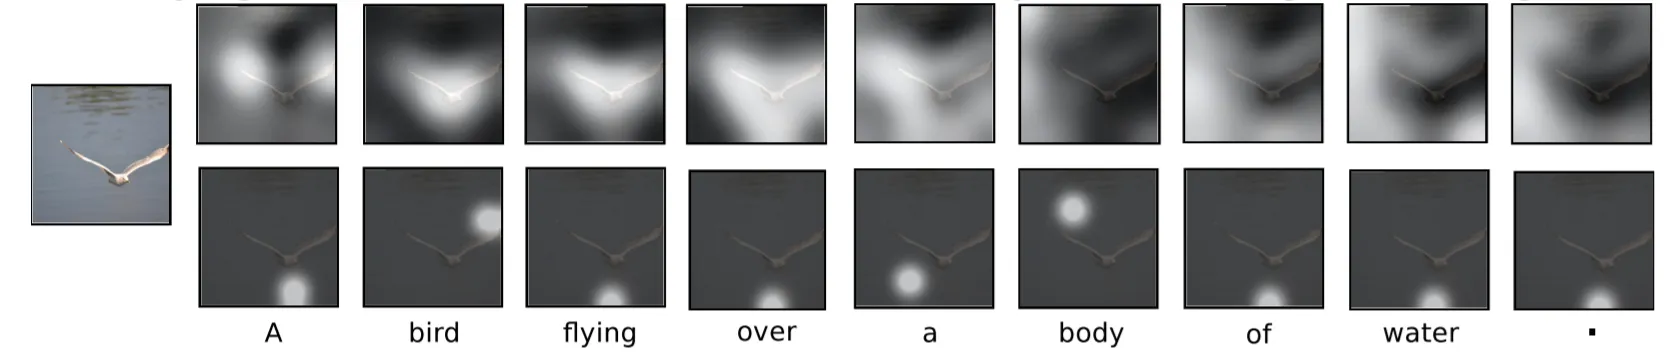
\includegraphics[width=\linewidth]{tikz/chapter7 - Attention Types.png}
    \caption{{\color{red}\colorbox{pink}{Tikz TO-DO}} Soft and Hard Attention}
\end{figure}

\section{Seq2Seq}

While significant breakthroughs initially emerged in image captioning, the most notable advancements took place in machine translation. Specifically, in 2016, Google introduced the first Neural Machine Translation model to enhance Google Translate.  Google achieved this not solely due to their resources but also thanks to influential academic works that preceded their efforts. One such influential work is  \href{https://arxiv.org/pdf/1409.3215}{"Sequence to Sequence Learning with Neural Networks" (Sutskever et al.)}, which shows the promise of Neural Machine Translation (NMT) over Statistical Machine Translation (SMT).

The distinguishing factor of this paper was the implementation of a machine translator in an end-to-end way. \textbf{End-to-end learning} means that the machine translator handles the entire translation process, from inputting the original text to outputting the translated text, without the need for separate components or intermediate steps. In order to do this, the model introduces for the first time the \textbf{encoder-decoder} approach to handle input sequences of variable lengths. 

\begin{enumerate}
    \item \textbf{Encoder}: LSTM that is responsible for mapping the variable length input phrase into a fixed-dimensional vector (\textbf{context vector}). The latter serves as a connection between the encoder and the decoder.
    \item \textbf{Decoder}: LSTM that maps the fixed vector into a variable length output sequence
\end{enumerate}

\begin{figure}[!htbp]
    \centering
    \includegraphics[width=\linewidth]{tikz/Seq2Seq.png}
    \caption{{\color{red}\colorbox{pink}{Tikz TO-DO}}}
\end{figure}

The image shows a very high prospective of the Seq2Seq model. The "c" block captures the entire input sequence. This limitation already suggest the need of an attention model, as the latent representation cannot contain all information about the entire input sequence.

\section{RNN Enc-Dec}
RNN Enc-Dec was introduced in the work \href{https://arxiv.org/pdf/1409.3215}{"Learning Phrase Representations using RNN Encoder-Decoder for Statistical Machine Translation" (Cho et al.)}, in which a context vector is used for word decoding.

\begin{figure}[!htbp]
    \centering
    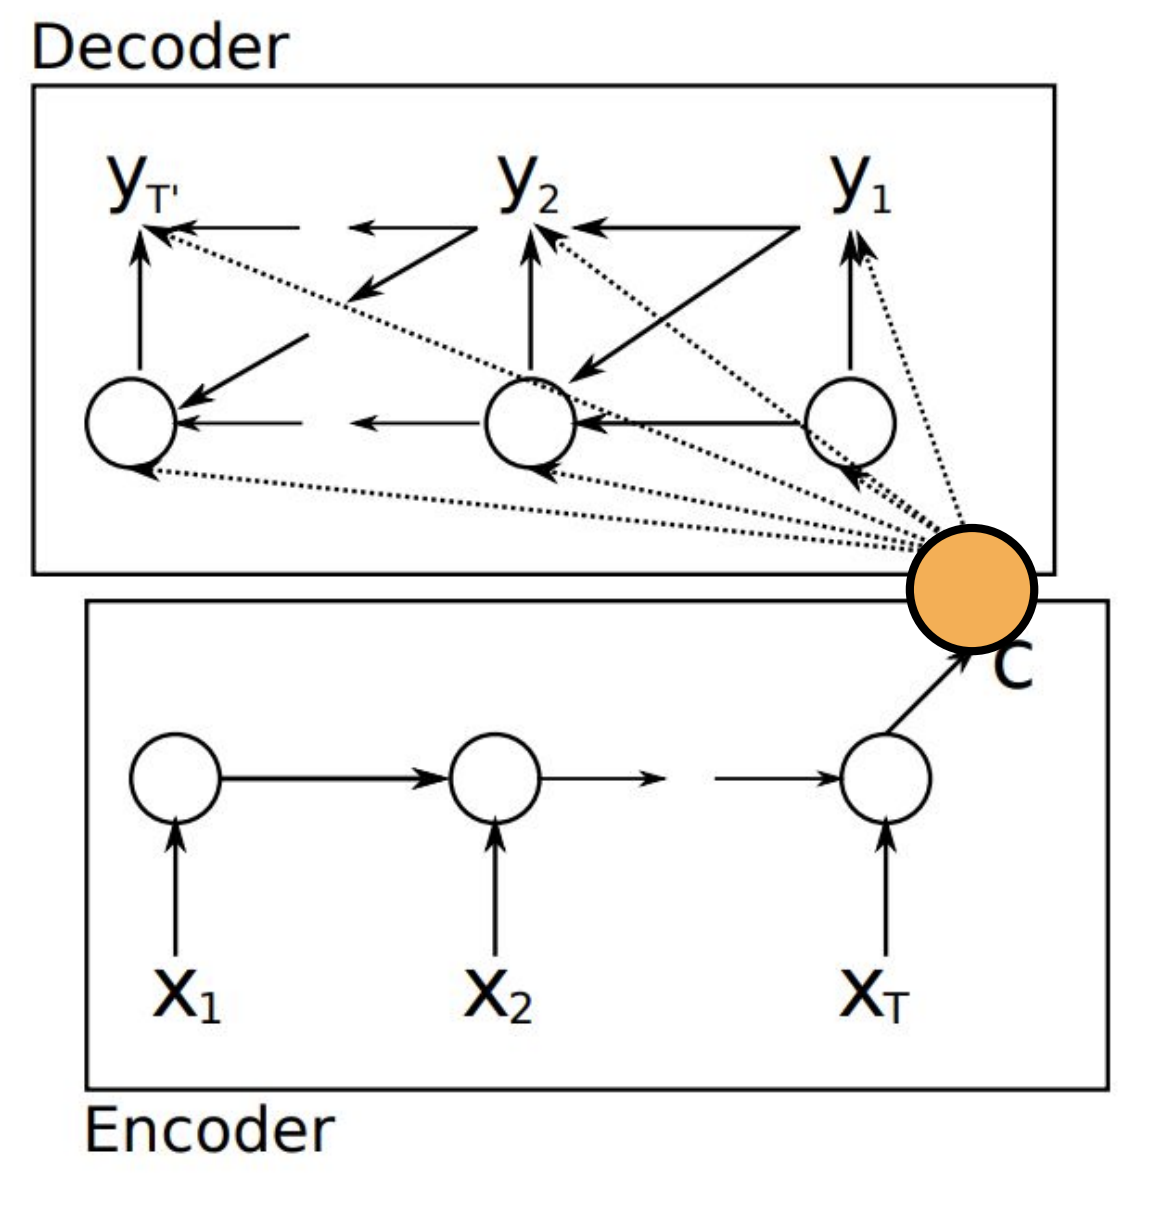
\includegraphics[width=0.45\linewidth]{tikz/chapter7 - RNN Enc-Dec.png}
    \caption{{\color{red}\colorbox{pink}{Tikz TO-DO}}  RNN Enc-Dec Architecture}
\end{figure}

The RNN Encoder-Decoder model is fundamentally identical to the Seq2Seq model, in that both follow the same principle of transforming a variable-length input sequence into a variable-length output sequence via a fixed-length vector representation, known as \textbf{context vector}. 

This approach requires the \textbf{encoder and decoder to be trained jointly}, which allows the model to learn a latent representation that depends on the context vector. A significant improvement of this model is the introduction of GRUs (Gated Recurrent Units), which offer advantages in computational efficiency and learning capability over traditional RNNs.

However, as before, a critical problem with this approach is the need to compress all relevant information in a source sentence into a fixed-length vector. This can be particularly difficult when \textbf{dealing with long sentences}, as the model may not be able to capture all the necessary information in a compact representation. As a result, the quality of the output sequence generated by the decoder may decrease as the length of the input sequence increases.

\section{RNN with attention}

Because of the above problem, the community realized that RNNs alone were not sufficient and that the integration of an attention module was needed. The same working group published the article \href{https://arxiv.org/pdf/1409.0473}{"Neural Machine Translation by Jointly Learning to Align and Translate" (Bahdanau et al.)}, in which the attention mechanism was introduced. 

In an RNN architecture with attention, the encoder is a \textbf{bidirectional LSTM}, which enhances latent representations for each input word. Indeed, every word is represented by a vector that is the concatenation of the hidden states of the LSTMs that read the sequence both left-to-right and right-to-left.

The decoder, on the other hand, generates the output sequence one step at a time, using the latent representations of the encoder and the dynamic context provided by the attention mechanism. \textbf{This context is not fixed}, but changes with each decoding step, allowing the decoder to "pay attention" to different parts of the input sequence depending on which part of the output it is generating. The context vector is modulated by attention variables $\alpha_{ti}$.

\begin{figure}[!htbp]
    \centering
    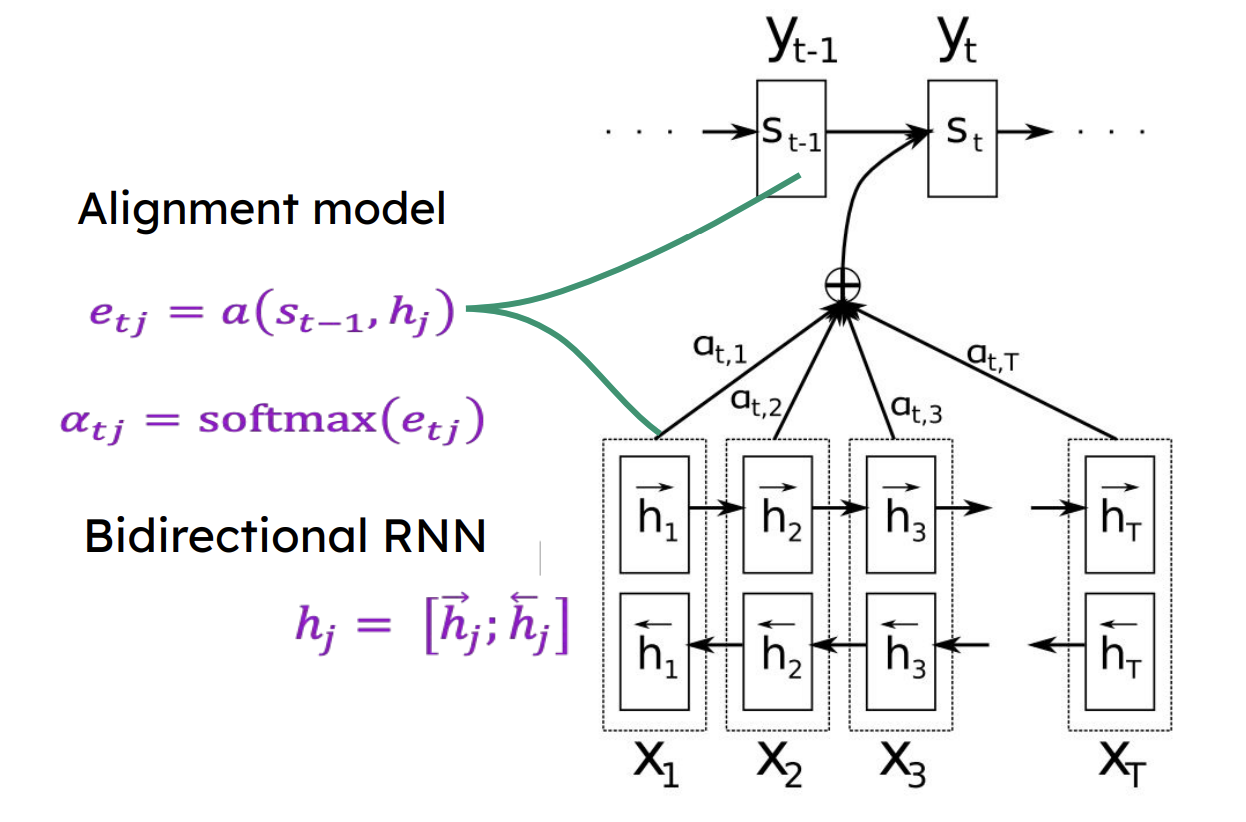
\includegraphics[width=0.7\linewidth]{tikz/chapter7 - RNN with Attention.png}
    \caption{{\color{red}\colorbox{pink}{Tikz TO-DO}} RNN with Attention Architecture}
\end{figure}


The attention mechanism works as follows:
\begin{enumerate}
    \item \textbf{Calculation of Latent Representations}:
    For each word in the input sequence, a latent representation $h_j$ is computed by concatenating the outputs of the bidirectional LSTM units:
    $$
    h_j=\left[ \overrightarrow{h_j}:\overleftarrow{h_j} \right]
    $$
    
    \item \textbf{Model Alignment}:
    When generating the output word at time $t$, an \textbf{alignment score} $e_{tj}$ is computed between the previous state of the decoder $s_{t-1}$ and \underline{each} latent representation $h_j$ of the input sequence:
    $$
       e_{tj} = a(s_{t-1}, h_j)
    $$
    The alignment model $a$ can be implemented with a simple neural network.
    \vspace{0.25cm}
    
    \item \textbf{Weights of Attention}:
    A softmax function is applied to the alignment scores to obtain the attention weights $\alpha_{tj}$:
    $$
       \alpha_{tj} = \text{softmax}(e_{tj})
    $$
    These weights represent the relative importance of each input word to the current output word.
    \vspace{0.25cm}
    
    \item \textbf{Calculation of Vector Context}:
    The vector context $c_t$ for time $t$ is calculated as a weighted sum of the latent representations, using the attention weights:
    $$
       c_t = \sum_{j=1}^{T}\alpha_{tj}h_j
    $$
    The embeddings of all inputs are multiplied by their respective attention scores (in practice, most scores are zero, while one or two might have a value such as 0.8 and 0.2, for example). Thus, the context vector is the \textbf{combination of all relevant inputs for the current output}.
    \vspace{0.25cm}
    
    \item \textbf{Generation of Output}:
    The context vector $c_t$ together with the previous state of the decoder $s_{t-1}$ is used to generate the next state of the decoder $s_t$ and the output word $y_t$.
\end{enumerate}


\begin{figure}[!htbp]
    \centering
    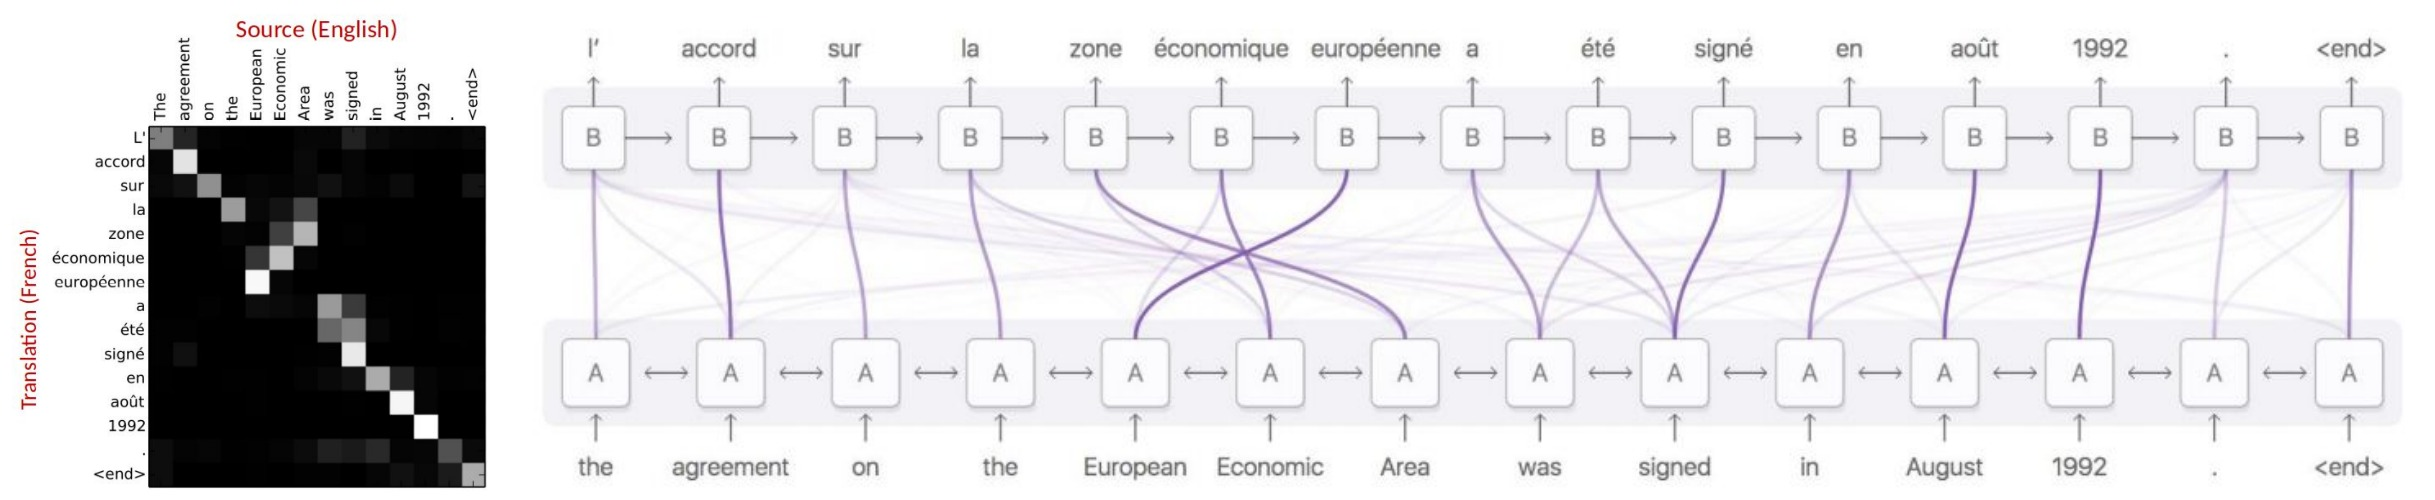
\includegraphics[width=\linewidth]{tikz/chapter7 - Attention is Alignment.jpg}
    \caption{{\color{red}\colorbox{pink}{Tikz TO-DO}} The mechanism of attention in the RNN Encoder-Decoder model}
\end{figure}

In the image above, the attention matrix on the left shows the alignment between the words in the input sequence (English) and the words in the output sequence (French) for an example sentence. The lines in the diagram on the right illustrate how the attention mechanism allows the decoder to directly access representations of the encoder states by dynamically focusing on the relevant parts of the input sequence.


\section{Local Attention}

The attention used in RNN Enc-Dec is called \textbf{global attention} because the module attends all of the inputs. Logically, this is a waste of resources and it can also be misleading. Research showed lately that best results where obtained with \textbf{local attention}, firstly introduced in the paper \href{https://arxiv.org/pdf/1508.04025}{"Effective Approaches to Attention-based Neural Machine Translation" (Luong et al.)}.

In local attention mechanisms, \textbf{the model focuses only on a subset of the input sequence}, rather than the entire sequence, to compute the context vector $c_t$. This subset is determined by an aligned position indication $p_t$, which the model learns during training based on the previous decoder state $s_{t-1}$.

Instead of using a global view of all input tokens, local attention utilizes a \textbf{position-based approach}. The aligned position $p_t$ determines a specific range or window around which the attention is concentrated. This approach allows the model to adapt dynamically to different parts of the input sequence, which can vary in relevance during the output generation process.

\begin{figure}[!htbp]
    \centering
    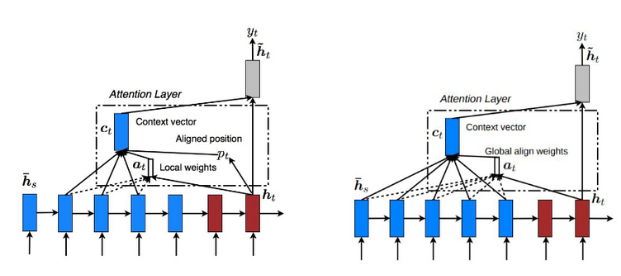
\includegraphics[width=\linewidth]{tikz/Local Attention comparison.png}
    \caption{{\color{red}\colorbox{pink}{Tikz TO-DO}} Global Attention vs. Local Attention}
\end{figure}

The image above shows a comparison between a global attention module (right) and a local attention module (left), illustrating the difference in focus areas for the input sequence during output generation.

The computation of local attention involves the following steps:

\begin{itemize}
    
    \item \textbf{Aligned Position Calculation}:
    To make backpropagation feasible, the aligned position $p_t$ is determined using a gating mechanism and is dependent on the previous decoder state $s_{t-1}$:
    $$
    p_t = L_s \cdot \sigma(v^T_p \tanh(W_p s_{t-1}))
    $$
    Here, $L_s$ represents the length of the input sequence, $\sigma$ denotes the sigmoid function, and $v_p$ and $W_p$ are learnable parameters.
    \vspace{0.25cm}
    
    \item \textbf{Attention Weights Calculation}:
    The attention weights $\alpha_{tj}$ are computed as a combination of soft attention and a proximity-based term, similar to a radial kernel:
    $$
    \alpha_{tj} = \text{softmax}(h_j^T W_a s_{t-1}) \cdot \exp\left(-\frac{(j - p_t)^2}{2\sigma^2}\right)
    $$
    This equation emphasizes words closer to the aligned position $p_t$, thereby creating a localized attention effect.
    \vspace{0.25cm}
    
    \item \textbf{Context Vector Calculation}:
    The context vector $c_t$ is computed as a weighted sum of the input representations $h_j$, using the attention weights $\alpha_{tj}$:
    $$\label{eq:local-attention}
    c_t = \sum_{j} \alpha_{tj} h_j
    $$
    
    \item \textbf{Decoder State Update}:
    Using $c_t$ and the previous decoder state $s_{t-1}$, the current state $\widetilde{s_t}$ of the RNN cell is updated:
    $$
    \widetilde{s_t} = \tanh(W_c [c_t; s_t])
    $$
    
    \item \textbf{Output Probability Calculation}:
    Finally, the probability distribution over the output vocabulary is computed using $\widetilde{s_t}$:
    $$
    p(y_t \mid y_{<t}, x) = \text{softmax}(W_s \widetilde{s_t})
    $$
    ($y_{<t}$ are all the output words generated up to the time $t-1$)

\end{itemize}


\section{GNMT (Google Neural Machine Translation)}

Having discussed the significant milestones in the field of Machine Translation, we are now prepared to delve into the Google Neural Machine Translation (GNMT) system, as introduced in \href{https://arxiv.org/pdf/1609.08144}{Schuster et al.'s paper, "Google's Neural Machine Translation System: Bridging the Gap between Human and Machine Translation"}. This remarkable architecture integrates all the previously mentioned components in an innovative manner. At a high level, GNMT consists of an encoder-decoder system with attention mechanisms. The attention model leverages latent representations learned by the encoder LSTM and those associated with the target words in the decoder. The decoder's output is then processed through a softmax layer.

\begin{figure}[!htbp]
    \centering
    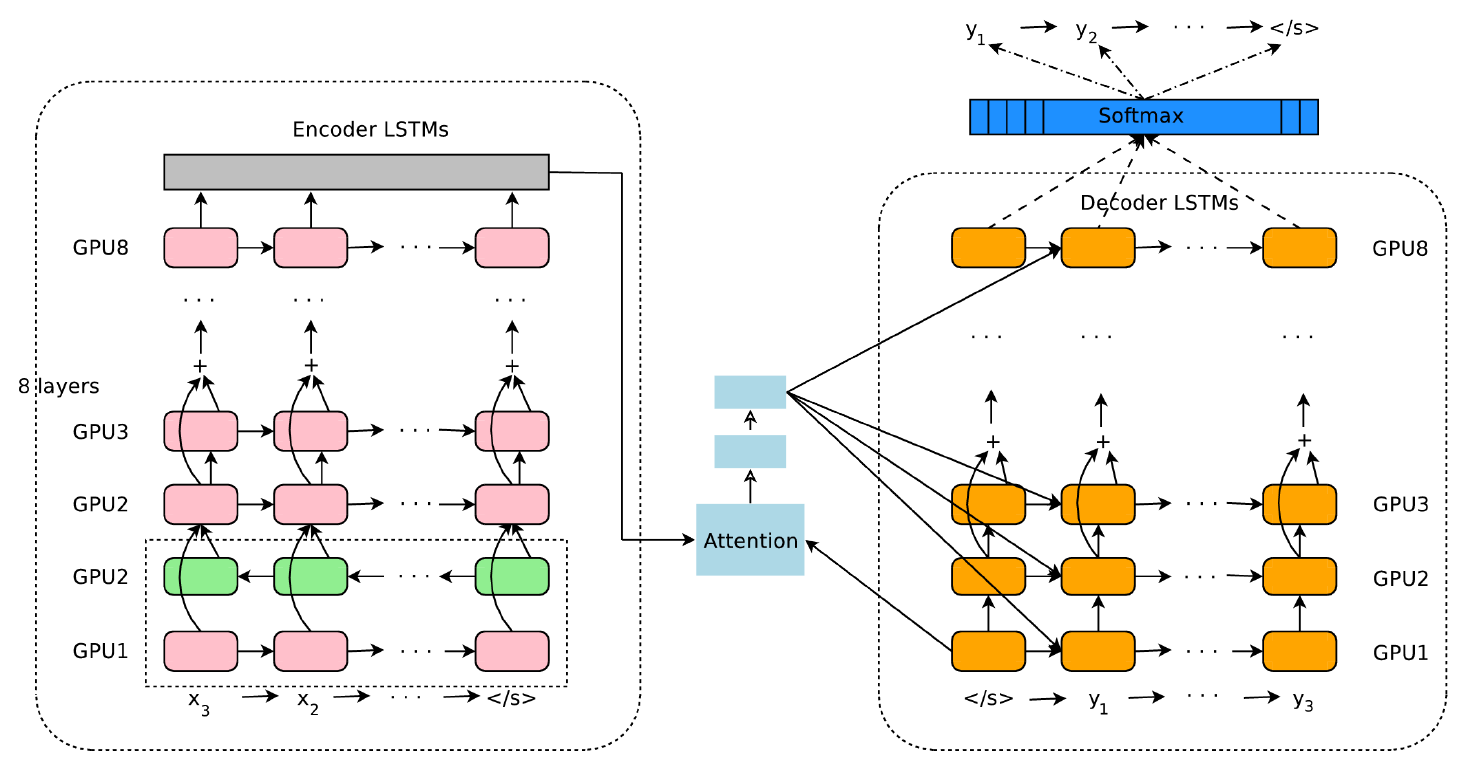
\includegraphics[width=1\linewidth]{tikz/chapter7 - GNMT.png}
    \caption{{\color{red}\colorbox{pink}{Tikz TO-DO}} GNMT Architecture}
\end{figure}

\textbf{Encoder Architecture}: The encoder is composed of several layers of LSTMs. It starts with bidirectional lower layers of LSTMs, followed by stacked unidirectional LSTMs. Jump connections are incorporated during stacking to facilitate training. The model is distributed over 8 GPUs, with the model divided into 8 parts, each on a different GPU. The bidirectional lower layers of the encoder compute in parallel first. Once both are finished, the unidirectional layers of the encoder can begin computation, each on a separate GPU. This approach uses stacked LSTMs with residual connections.

\textbf{Decoder Architecture}: As far as the decoder is concerned, only the output of the lower layer is used to derive the attention context, which is then directly fed to all the upper layers of the decoder. Training is optimized using a loss function that improves the BLEU score, thus ensuring better quality of machine translation.


\section{Appendix - Word Embeddings}

\textit{Because we are thoughtful authors, we also add this tidbit: word embeddings!}

Computers are not able to comprehand raw words (ma dai!). For example, the word "drug" has no meaning for my beutifull laoptop. \footnote{I'm reviewing the section and I'm not sure if Jacopo was writing or having a seizure. \emoji{face-with-raised-eyebrow} - Fede} Therefore, \textbf{any task aimed at processing language} must begin with the essential representation of words.

A preliminary method is the \textbf{"bag of words"} model, which encodes words using a "one-hot" pattern. If our dataset contains sentences such as "I like the new movie!" and "I love the weather." we can represent the words as vectors:

\vspace{-1cm}
\begin{minipage}[t]{0.45\textwidth}
\begin{align*}
\text{"I"} \quad &[1,0,0,0,0,0,0] \\
\text{"like"} \quad &[0,1,0,0,0,0,0] \\
\text{"the"} \quad &[0,0,1,0,0,0,0] \\
\text{"new"} \quad &[0,0,0,1,0,0,0] \\
\text{"movie"}\quad  &[0,0,0,0,1,0,0] \\
\text{"love"} \quad &[0,0,0,0,0,1,0] \\
\text{"time"} \quad &[0,0,0,0,0,0,1]
\end{align*}
\end{minipage}
\begin{minipage}[t]{0.45\textwidth}
\vspace{2cm}
\begin{center}
The sentences will then be represented as $[1,1,1,1,1,0,0]$ and $[1,0,1,0,0,1,1]$.
\end{center}
\end{minipage}
\begin{minipage}[t]{0.1\textwidth}
\end{minipage}

However, as is evident, this representation is not effective in showing semantic relationships between words, as each is encoded as an individual entity in a vector space and there is no way to establish that the words "love" and "like" have similar connotations. This is where word embeddings come in.

\textbf{Word embeddings} are representations in which contexts and similarities are captured by encoding in vector space. Similar words will have similar representations. \textbf{Word2Vec techniques} create a representation of each word in our vocabulary in a vector. Words used in similar contexts or that have semantic relationships are effectively captured through their \textbf{vicinity in vector space}. Embeddings create semantic and syntactic relationships between words. These relationships, or weights, are determined by the model and not pre-assigned (see example in the figure below).

\begin{figure}[!htbp]
        \centering
        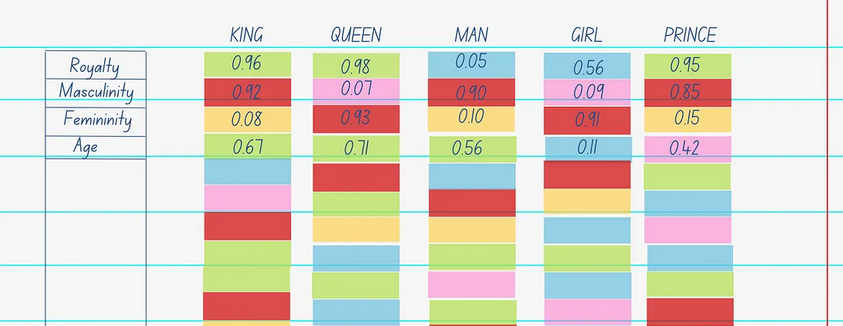
\includegraphics[width=0.8\linewidth]{tikz/Word2Vec example.png}
        \caption{{\color{red}\colorbox{pink}{Tikz TO-DO}} Word Embeddings Example}
\end{figure}

The image shows hypothetical features (weights) in word embeddings learned by the neural network. Consider a classic example: "king," "queen," "man," "girl," "prince." In a hypothetical world, vectors could then define the weight of each criterion (e.g., nobility, masculinity, femininity, age, etc.) for each of the words provided in our vocabulary. For example, "king," "queen," and "prince" have similar scores for "nobility," while "girl" and "queen" have similar scores for "femininity".

The architecture of Word2Vec is essentially a \textbf{two-layer surface neural network} trained to represent words in a document or text context. During training, the input consists of all the documents or texts in the training set, each of which is represented using a \textbf{one-hot encoding of the words} present. This means that each word is represented by a vector in which a single dimension is set to 1 and all others to 0, indicating the presence of the word in the document.

\begin{figure}[!htbp]
    \centering
    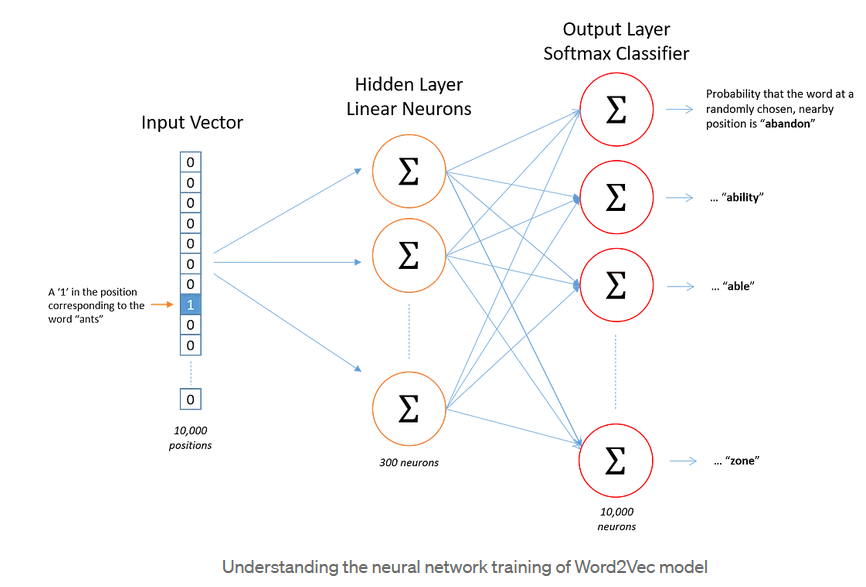
\includegraphics[width=0.8\linewidth]{tikz/W2V architecture.png}
    \caption{{\color{red}\colorbox{pink}{Tikz TO-DO}} Understanding the neural network training of Word2Vec model}
\end{figure}

The hidden layer of the neural network has a \textbf{number of neurons equal to the desired size for word embedding}. For example, if you want each word to be represented by a vector of length 300, the hidden layer will contain 300 neurons. During the training process, the weights associated with the hidden layers of the network are treated as the word embedding. These weights represent network parameters that capture the semantic and syntactic features of words, allowing them to be placed in a vector space in which similar words are close to each other. In other words, each word can be viewed as having a set of weights (300 in the case of the example) that "weigh" different semantic and syntactic features, such as the context in which they appear and their relationships to other words in the text.

Eventually, we can train a neural network to assign weights to each word embedding. The new weights on connections from inputs to activation features are the \textbf{Word Embeddings}.






